\documentclass[border=4pt]{standalone}
\usepackage{amsmath,amssymb}
\usepackage{tikz}
\usetikzlibrary{shadows,calc}
\begin{document}
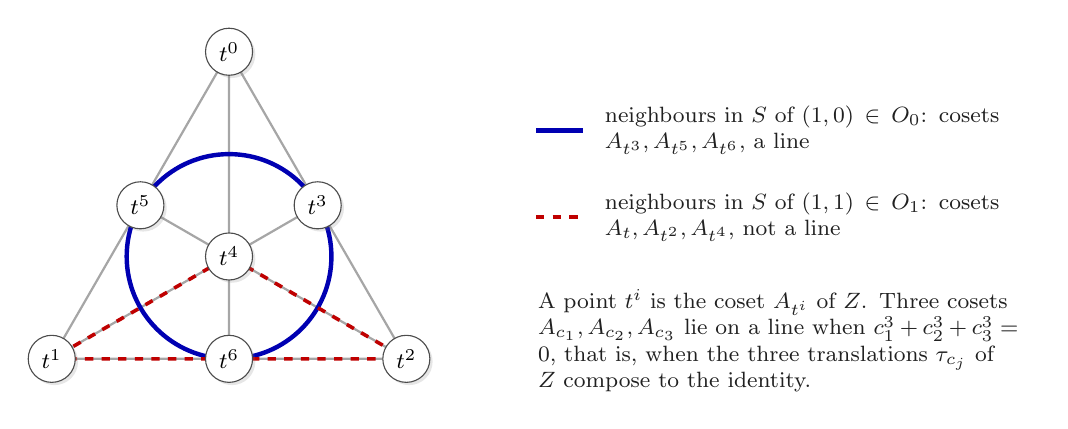
\begin{tikzpicture}[
  pt/.style={circle,draw=black!70,fill=white,inner sep=1.5pt,minimum size=17pt,font=\footnotesize,
             drop shadow={opacity=0.2,shadow xshift=1pt,shadow yshift=-1pt}},
  ln/.style={gray!70,thick},
  note/.style={font=\footnotesize,gray!25!black,align=left}]
  \def\R{2.6}
  \coordinate (V1) at (90:\R);
  \coordinate (V2) at (210:\R);
  \coordinate (V3) at (330:\R);
  \coordinate (M12) at ($(V1)!0.5!(V2)$);
  \coordinate (M23) at ($(V2)!0.5!(V3)$);
  \coordinate (M13) at ($(V1)!0.5!(V3)$);
  \coordinate (C) at (0,0);
  % the seven lines
  \draw[ln] (V1) -- (V2) -- (V3) -- cycle;
  \draw[ln] (V1) -- (M23) (V2) -- (M13) (V3) -- (M12);
  % the circle {3,5,6}, a line, is the S-neighbourhood of (1,0) in O_0
  \draw[blue!70!black,line width=1.6pt] (C) circle (0.5*\R);
  % the triangle {1,2,4}, not a line, is the S-neighbourhood of (1,1) in O_1
  \draw[red!75!black,line width=1.3pt,dashed] (V2) -- (V3) -- (C) -- cycle;
  \node[pt] at (V1)  {$t^0$};
  \node[pt] at (V2)  {$t^1$};
  \node[pt] at (V3)  {$t^2$};
  \node[pt] at (M12) {$t^5$};
  \node[pt] at (M23) {$t^6$};
  \node[pt] at (M13) {$t^3$};
  \node[pt] at (C)   {$t^4$};
  \begin{scope}[shift={(3.9,1.6)}]
    \draw[blue!70!black,line width=1.6pt] (0,0) -- (0.6,0);
    \node[note,anchor=west,text width=5.4cm] at (0.75,0)
      {neighbours in $S$ of $(1,0)\in O_0$: cosets $A_{t^3},A_{t^5},A_{t^6}$, a line};
    \draw[red!75!black,line width=1.3pt,dashed] (0,-1.1) -- (0.6,-1.1);
    \node[note,anchor=west,text width=5.4cm] at (0.75,-1.1)
      {neighbours in $S$ of $(1,1)\in O_1$: cosets $A_{t},A_{t^2},A_{t^4}$, not a line};
    \node[note,anchor=north west,text width=6.1cm] at (-0.1,-1.9)
      {A point $t^i$ is the coset $A_{t^i}$ of $Z$. Three cosets $A_{c_1},A_{c_2},A_{c_3}$ lie on a line when $c_1^3+c_2^3+c_3^3=0$, that is, when the three translations $\tau_{c_j}$ of $Z$ compose to the identity.};
  \end{scope}
\end{tikzpicture}
\end{document}
